\documentclass{article}

\usepackage{graphicx}
\usepackage{tikz}
\usepackage{tikzsymbols}
\usetikzlibrary{calc,patterns,shapes.geometric}
\pagestyle{empty}
\usepackage[margin=0pt]{geometry}
\geometry{papersize={14in,12in}}

\def\centerarc[#1](#2)(#3:#4:#5){\draw[#1] ($(#2)+({#5*cos(#3)},{#5*sin(#3)})$) arc (#3:#4:#5);}

\begin{document}
	\begin{figure}
		\centering
		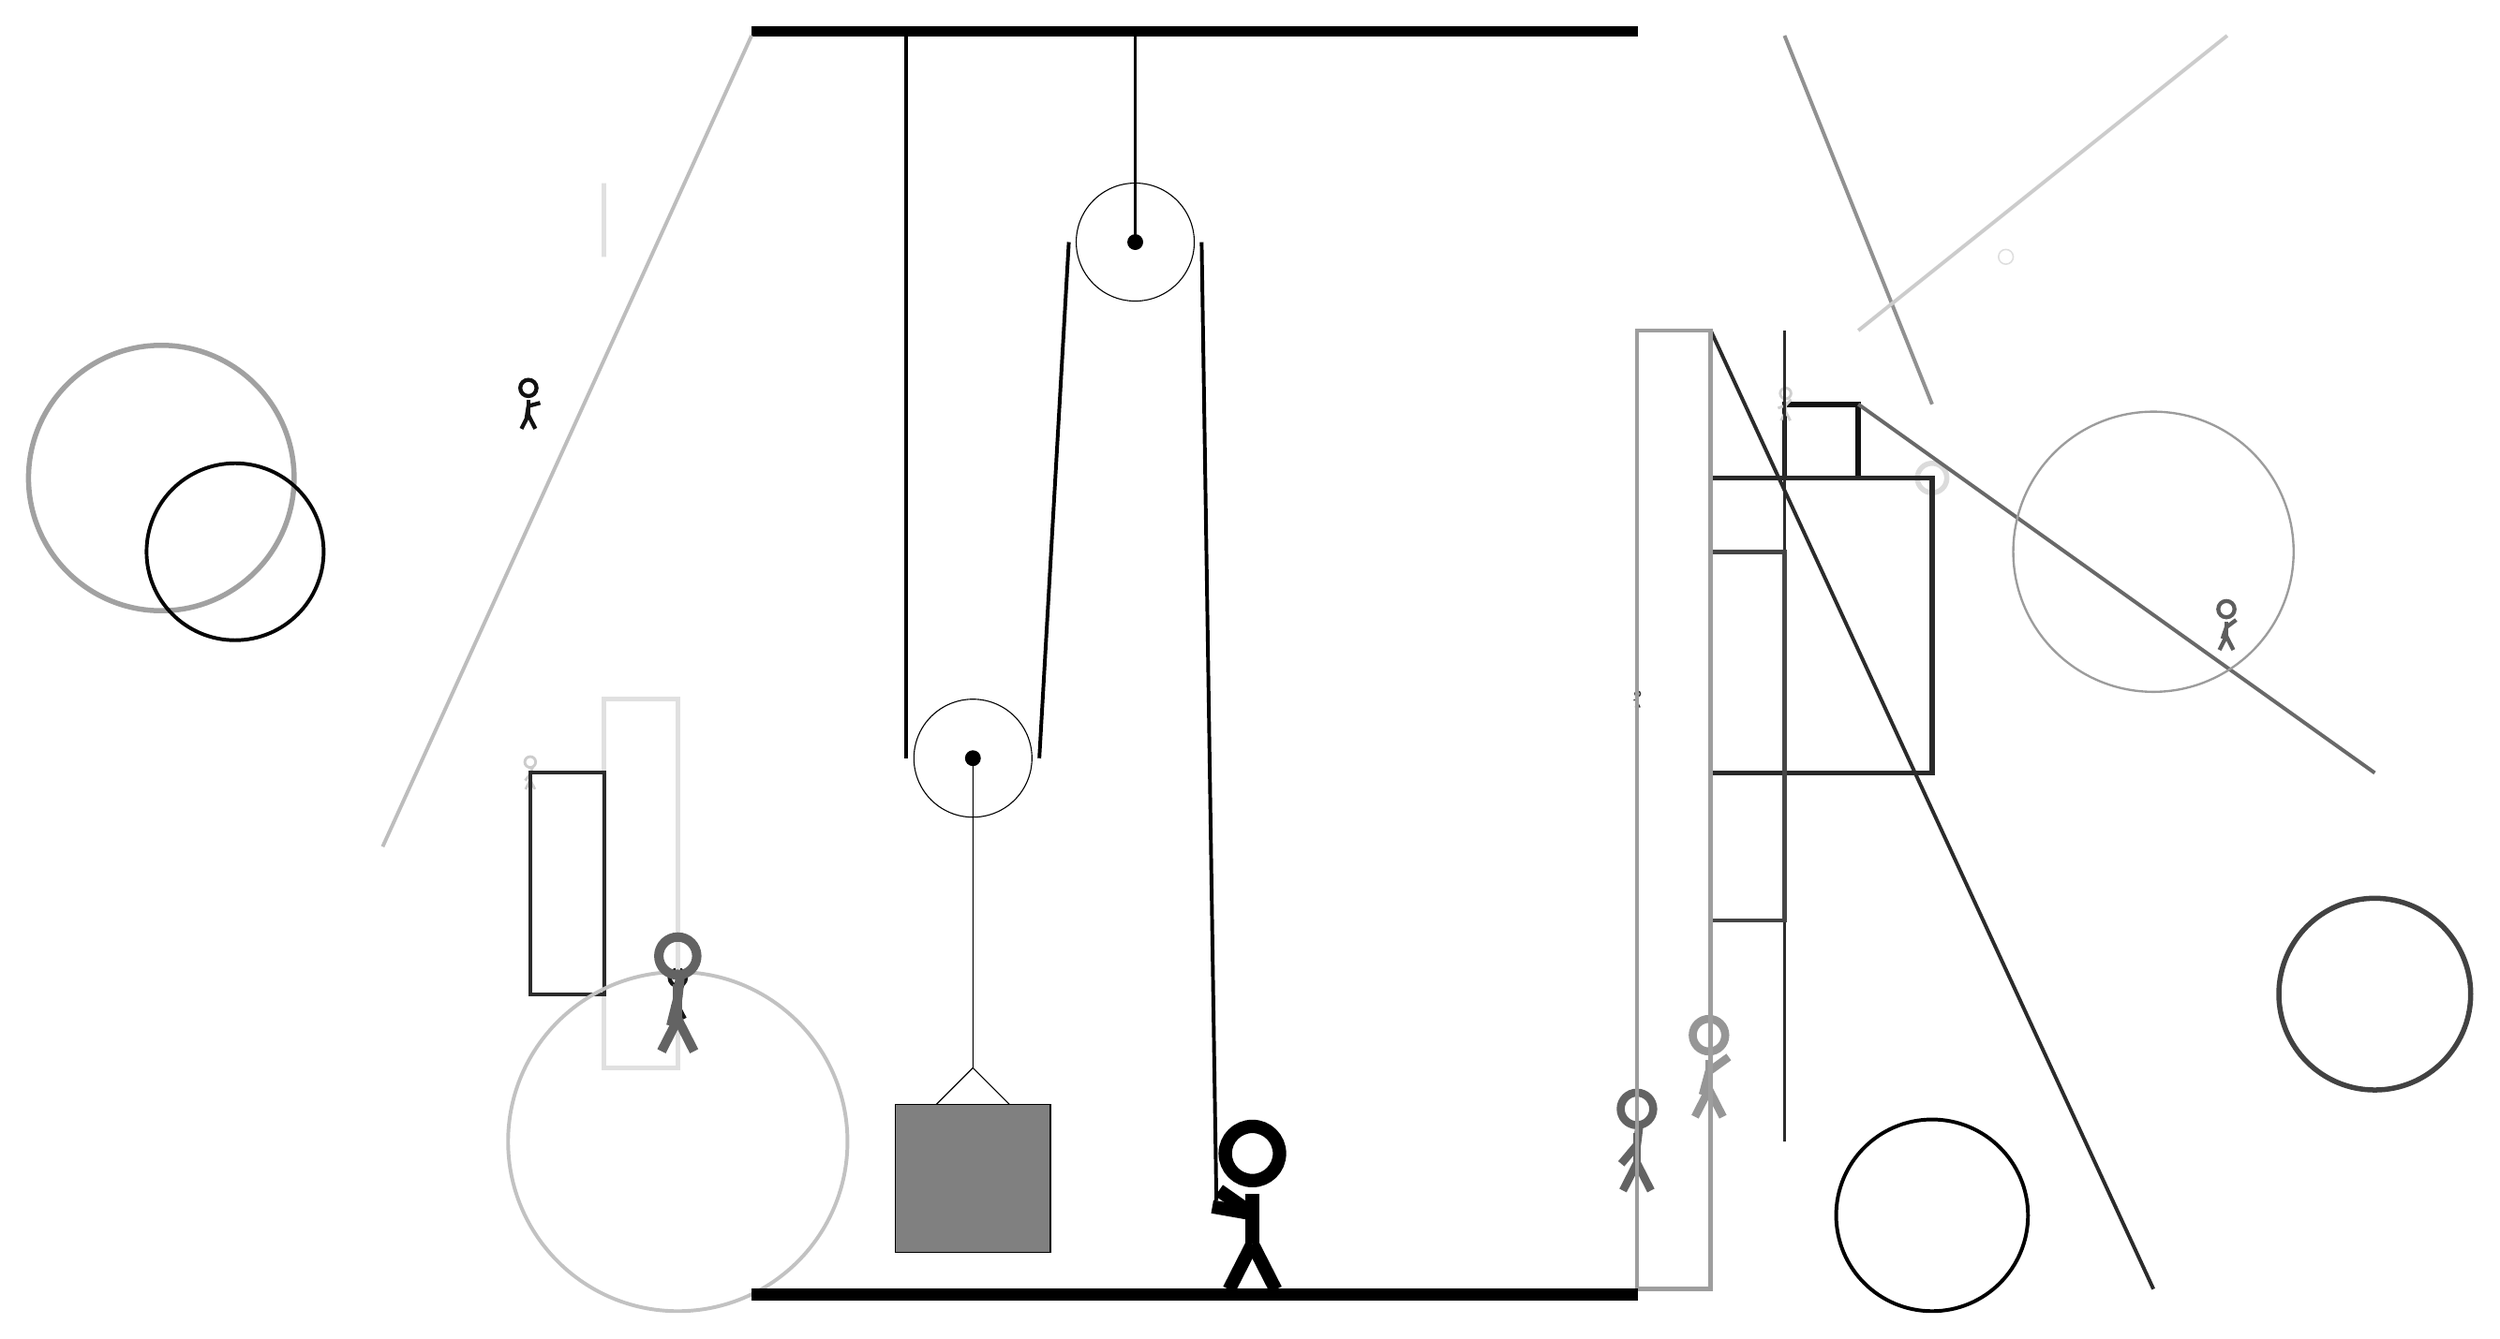
\begin{tikzpicture}
			%%%%% START %%%%%
			
			\draw[fill=black] (-2, 14) rectangle (10, 14.125);
			
			\draw (3.2, 11.2) circle (0.8);
			\draw[fill=black] (3.2, 11.2) circle (0.1);
			\draw[thick] (3.2, 11.2) -- (3.2, 14);
			
			\draw (1, 4.2) circle (0.8);
			\draw[fill=black] (1, 4.2) circle (0.1);
			
			\draw (1, 4.2) -- (1, 0) -- (0.5, -0.5);
			\draw (1, 0) -- (1.5, -0.5);
			\draw[fill=black!50] (-0.05, -0.5) rectangle (2.05, -2.5);
			
			\draw[line width=0.5mm] (0.1, 14) -- (0.1, 4.2);
			\centerarc[line width=0.5mm](1, 4.2)(180:360:0.9);
			\draw[line width=0.5mm](1.9, 4.2) -- (2.3, 11.2);
			\centerarc[line width=0.5mm](3.2, 11.2)(0:180:0.9);
			\draw[line width=0.5mm](4.1, 11.2) -- (4.3, -1.8);
			
			\node at (4.7, -1.9) {\Strichmaxerl[10][-35][170]};
			
			\draw[line width=0.7mm, color=black!93] (12, 9) rectangle (13, 8);
			
			\draw[line width=0.5mm, color=black!43](14, 9) -- (12, 14);
			\draw [line width=0.7mm, color=black!37](-10, 8) circle (1.8);
			\draw [line width=0.7mm, color=black!14](14, 8) circle (0.2);
			\node[line width=0.2mm, color=black!91] at (-3, 1) {\Strichmaxerl[3][66][67]};
			\draw [line width=0.5mm, color=black!98](-9, 7) circle (1.2);
			\draw [line width=0.7mm, color=black!74](20, 1) circle (1.3);
			\node[line width=0.2mm, color=black!93] at (-5, 9) {\Strichmaxerl[3][81][15]};
			\draw[line width=0.7mm, color=black!12] (-4, 0) rectangle (-3, 5);
			\node[line width=0.5mm, color=black!20] at (-5, 4) {\Strichmaxerl[2][52][71]};
			
			\node[line width=0.7mm, color=black!61] at (10, -1) {\Strichmaxerl[6][50][83]};
			
			\draw[line width=0.5mm, color=black!59](13, 9) -- (20, 4);
			\draw [line width=0.2mm, color=black!13](15, 11) circle (0.1);
			
			\node[line width=0.4mm, color=black!19] at (12, 9) {\Strichmaxerl[2][19][47]};
			\draw[line width=0.5mm, color=black!20](13, 10) -- (18, 14);
			\draw[line width=0.5mm, color=black!83] (-4, 4) rectangle (-5, 1);
			
			\draw[line width=0.6mm, color=black!84] (10, 4) rectangle (10, 2);
			\node[line width=0.2mm, color=black!81] at (10, 5) {\Strichmaxerl[1][3][87]};
			\draw[line width=0.4mm, color=black!83] (12, 10) rectangle (12, -1);
			\node[line width=0.2mm, color=black!63] at (18, 6) {\Strichmaxerl[3][71][37]};
			\draw[line width=0.7mm, color=black!84] (11, 8) rectangle (14, 4);
			
			\node[line width=0.3mm, color=black!41] at (11, 0) {\Strichmaxerl[6][75][36]};
			
			\draw[line width=0.5mm, color=black!83](11, 10) -- (17, -3);
			\draw[line width=0.5mm, color=black!26](-7, 3) -- (-2, 14);
			\draw[line width=0.6mm, color=black!73] (12, 7) rectangle (11, 2);
			
			\draw [line width=0.3mm, color=black!39](17, 7) circle (1.9);
			\draw[line width=0.7mm, color=black!12] (-4, 12) rectangle (-4, 11);
			\draw[line width=0.6mm, color=black!38] (11, -3) rectangle (10, 10);
			\draw [line width=0.5mm, color=black!24](-3, -1) circle (2.3);
			
			\draw [line width=0.5mm, color=black!100](14, -2) circle (1.3);
			\node[line width=0.7mm, color=black!61] at (-3, 1) {\Strichmaxerl[7][76][84]};
			
			
			\draw[fill=black] (-2, -3) rectangle (10, -3.15);
			
			%%%%% END %%%%%
		\end{tikzpicture}
	\end{figure}	
\end{document}